\section{Result and Evaluation} \label{sec:eval}
This section discuss the result of the simulation with our implemented lattice Boltzmann method on SpiNNaker. Firstly, the evaluation setup (\ref{sec:es}) including the serial version and SpiNNaker version would be discussed. Then we will discuss the correctness and the accuracy of simulation in different scale at \ref{sec:caae}. Then we will compare the performance in term of speed with the serial implementation in CPU at \ref{sec:perfe}.
\subsection{Evaluation Setup} \label{sec:es}
In this project, we used a serial implementation of the test problem in C as the baseline. The serial version would be run on EPCC's facility Cirrus (Intel Xeon E5-2695 (Broadwell)), with no compiler optimization.\\

On the SpiNNaker side, we run our simulation on the SpiNNaker cluster in the University of Manchester, which contains 1,036,800 cores via the SpiNNaker Jupyter Notebook interface. \\

For evaluation, we use three different scale of simulation; see \ref{table:setting}. We will firstly plot the contour graph of the result of those three simulation. Those simulation indicate the same problem but in different resolution. Then we will use the normalized distances L-1 norm, L-2 norm and L-infinite norm  of (1) SpiNNaker version vs. Serial float version; (2) SpiNNaker version vs. Serial double version; (3) Serial float version vs. Serial double version to discuss the correctness and the accuracy of our SpiNNaker implementation.\\

\begin{table}[tb]
\centering
\begin{tabular}{|c|c|c|c|}
\hline
Scale          & 64$\times$64 & 128$\times$128 & 256$\times$256 \\ \hline
total cores    & 4086         & 16384          & 65536          \\ \hline
total timestep  & 5120         & 10240          & 20480          \\ \hline
$\nu$           & 0.000064     & 0.000128       & 0.000256       \\ \hline
$\tau$           & 0.500192     & 0.500384       & 0.500735       \\ \hline
\end{tabular}
\caption{The physical parameters setting in three different scales.}
\label{table:setting}
\end{table}


For performance, in this project, we focus on speed. To more visually compare the magnitude of the relationship between them, after confirmed the correctness, we do not take physical settings into consideration. In other words, all the experiments of those three scale would run for 12000 time steps. We will compare the total simulation time and the simulation time per time step of the SpiNNaker implementation and serial implementation in the three scales. \\

It should be noted that, in SpiNNaker, we do not take the time spend on loading SpiNNaker hardware configuration into account for the above comparison. We will discuss it in more detail at \ref{sec:ana}.\\

To make the results more plausible, we took the tie value for three executions for every result.\\
\subsection{Correctness and Accuracy Evaluation} \label{sec:caae}
Firstly, we can get an general judgement on the correctness from the vorticity contour. In Fig.~\ref{fig:contour}, Fig.~\ref{fig:a},Fig.~\ref{fig:c} and Fig.~\ref{fig:e} is produced from the serial C implementation in double floating precise. According to \cite{minion1997performance}, with its configuration, there would be a turbulence in the periodic system. It is clear that there are turbulence in all three scale. Turbulence is recognized as a complex system and if there is any small error during the calculation, eventually, the result would be markedly different. In this case, we got a similar turbulence as \cite{minion1997performance}; and now We are confident enough that our serial implementation is correct.\\

On the left hand side of \ref{fig:contour}, we have the contour result from the SpiNNaker implementation. It is clear that the result from the SpiNNaker implementation has similar contours as the serial C implementation. We can now say that our implementation is correct. However, CFD need accuracy and if we want to know how accurate our simulation is, we need to analysis the result numerically.\\

\begin{figure}[htbp]  
\begin{subfigure}{0.43\textwidth}
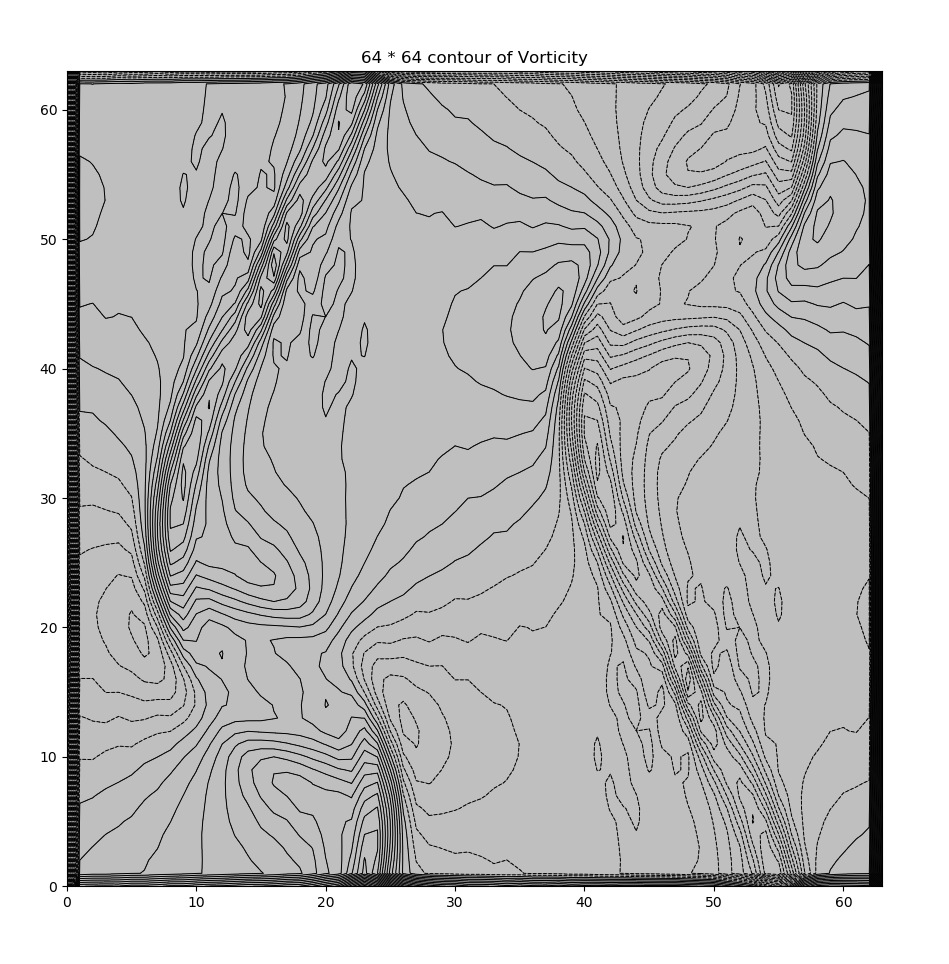
\includegraphics[width=\linewidth]{figures/double_c_64.png}
\caption{Contour of 64$\times$64 from serial C implementation} \label{fig:a}
\end{subfigure}\hspace*{\fill}
\begin{subfigure}{0.57\textwidth}
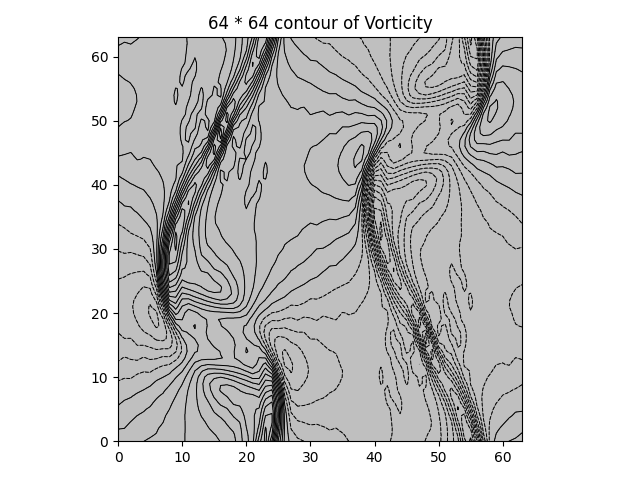
\includegraphics[width=\linewidth]{figures/spinnaker_64.png}
\caption{Contour of 64$\times$64 from SpiNNaker implementation} \label{fig:b}
\end{subfigure}

\medskip
\begin{subfigure}{0.43\textwidth}
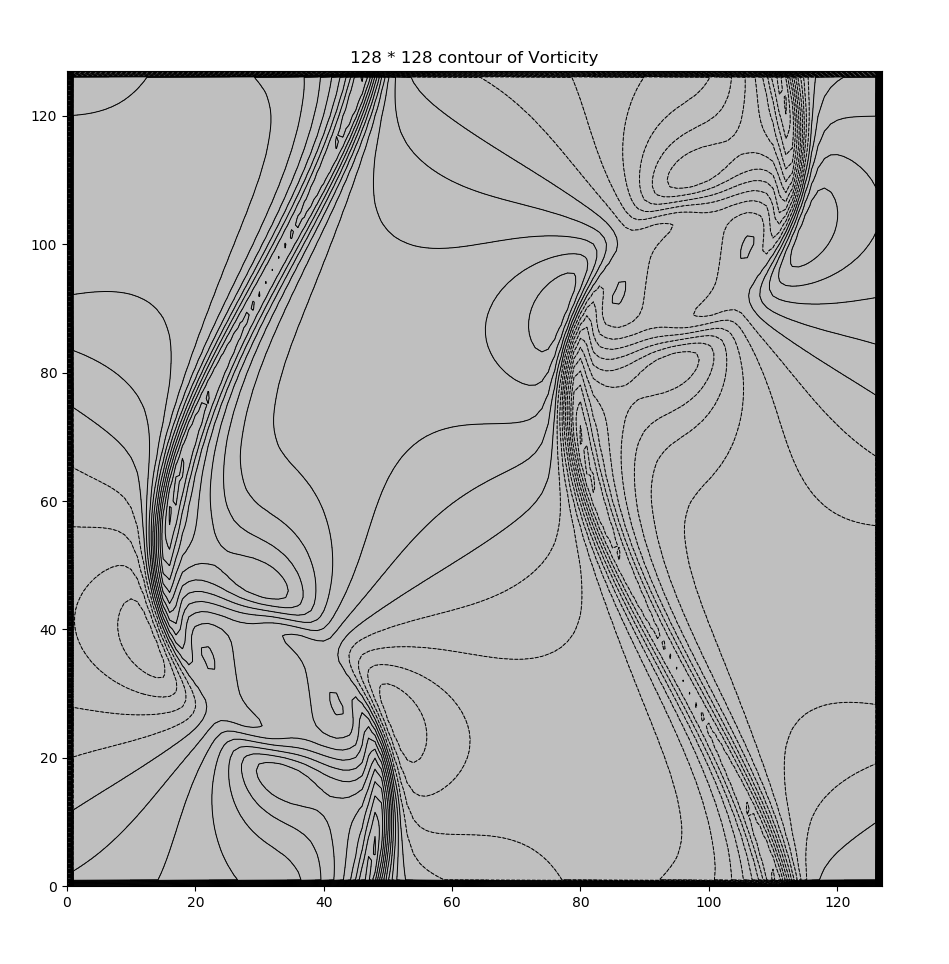
\includegraphics[width=\linewidth]{figures/double_c_128.png}
\caption{Contour of 128$\times$128 from serial C implementation} \label{fig:c}
\end{subfigure}\hspace*{\fill}
\begin{subfigure}{0.57\textwidth}
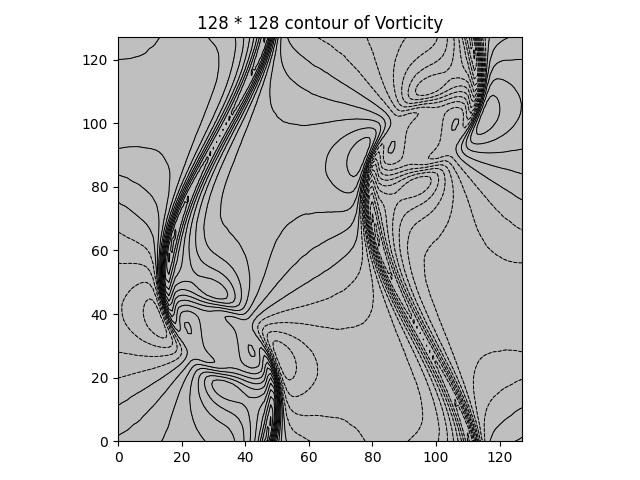
\includegraphics[width=\linewidth]{figures/spinnaker_128.png}
\caption{Contour of 64$\times$64 from SpiNNaker implementation} \label{fig:d}
\end{subfigure}

\medskip
\begin{subfigure}{0.43\textwidth}
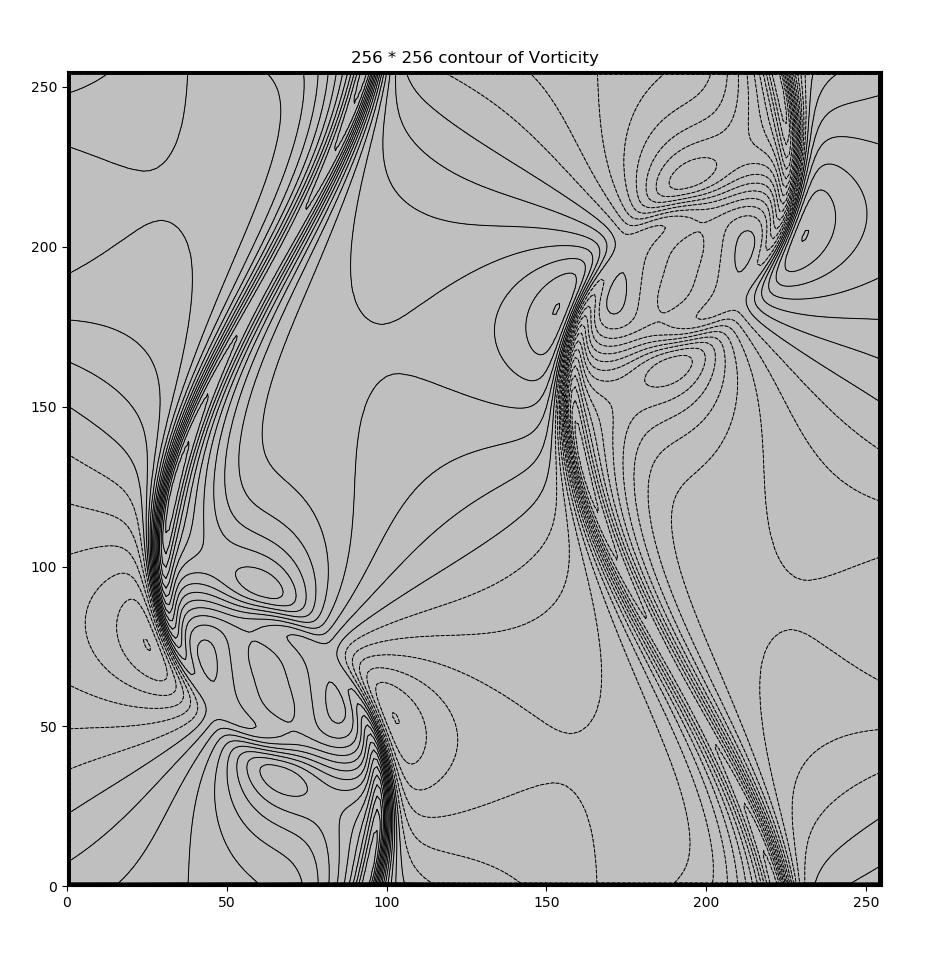
\includegraphics[width=\linewidth]{figures/double_c_256.png}
\caption{Contour of 256$\times$256 from serial C implementation} \label{fig:e}
\end{subfigure}\hspace*{\fill}
\begin{subfigure}{0.57\textwidth}
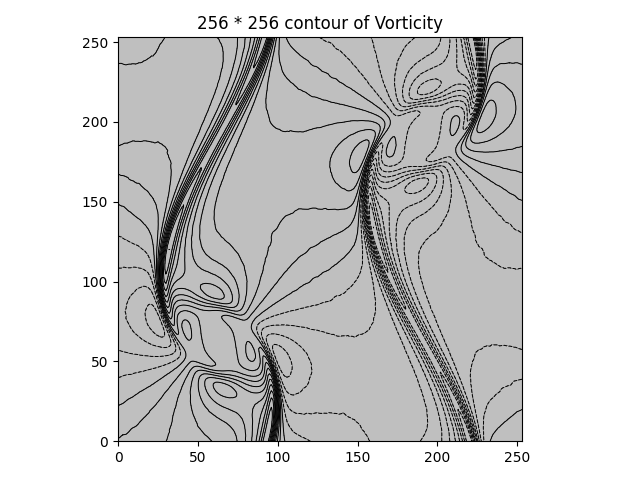
\includegraphics[width=\linewidth]{figures/spinnaker_256.png}
\caption{Contour of 64$\times$64 from SpiNNaker implementation} \label{fig:f}
\end{subfigure}
\caption{Contour graphs of the simulations in three different scale. \ref{fig:a},\ref{fig:c},\ref{fig:e} are the contour graph with scale of $32\times32$, $64\times64$ and $128\times128$ from serial C implementation in double floating precise.\ref{fig:b},\ref{fig:d},\ref{fig:f} are the contour graph with scale of $32\times32$, $64\times64$ and $128\times128$ from SpiNNaker implementation.} 
\label{fig:contour}
\end{figure}

In Table.~\ref{table:norm}, we show how we quantifying the variation between different results. We can regard the double precis serial C version as a baseline and compare it with the floating-point implementation in serial C. From the table, it is clear that in terms of $L-$ norm, $L-2$ norm and $L_{infi}$, SpiNNaker implementation maintained at the same level as C. More specifically, we introduced another criteria, the L-2 norm per grid, to quantify effect of error on each grid; and the L-2 per grid of SpiNNaker implementation also stay at the same level of floating-point C implementation. Therefore, we can confirm that, in terms of accuracy, SpiNNaker's LBM implementation is already at the level of existing CPUs.\\

\begin{table}[tb]
\begin{tabular}{|c|c|c|c|c|}
\hline
Scale                & Norm        & float vs. double& float vs. SpiNNaker& double vs. SpiNNaker\\ \hline
\multirow{4}{*}{64}  & L-1          & 0.003145             & 0.004472              & 0.003632               \\ \cline{2-5} 
                     & L-2          & 6.3365e-05           & 9.133678e-05          & 7.513214e-05           \\ \cline{2-5} 
                     & $L_{infi}$  & 4.2000e-06           & 6.600575e-06          & 5.867303e-06           \\ \cline{2-5} 
                     & L-2 per Grid & 1.54700e-08          & 2.22990e-08           & 1.83428e-08            \\ \hline
\multirow{4}{*}{128} & L-1          & 0.012635             & 0.013630              & 0.015220               \\ \cline{2-5} 
                     & L-2          & 0.000126             & 0.044751              & 0.000152               \\ \cline{2-5} 
                     & $L_{infi}$  & 4.50000e-06          & 4.416680e-06          & 5.739052e-06           \\ \cline{2-5} 
                     & L-2 per Grid & 7.69043e-08          & 2.73138e-06           & 9.27734e-09            \\ \hline
\multirow{4}{*}{256} & L-1          & 0.047357             & 0.056009              & 0.032206               \\ \cline{2-5} 
                     & L-2          & 0.000239             & 0.000278              & 0.000142               \\ \cline{2-5} 
                     & $L_{infi}$  & 4.300000e-06         & 4.80000e-06           & 9.000001e-06           \\ \cline{2-5} 
                     & L-2 per Grid & 1.4296e-08           & 1.7792e-08            & 9.088e-09              \\ \hline
\end{tabular}
\caption{A chart of three different matrix norm between each two of floating-point C, double precis floating-point C and SpiNNaker. Here we use L-1 norm, L-2 norm and L-infinite norm to quantify the extent of variation in results. Besides, we introduce another criteria L-2 norm per grid to quantify the variation of each lattice.}
\label{table:norm}
\end{table}

\subsection{Performance Evaluation} \label{sec:perfe}
After quantifying the correctness and the accuracy, we now have a reasonably correct implementation. Then To make it easier to measure its performance, we execute the simulation with different scale in the same time step i.e. 12000 steps.\\

\begin{figure}[tb]
   \centering
       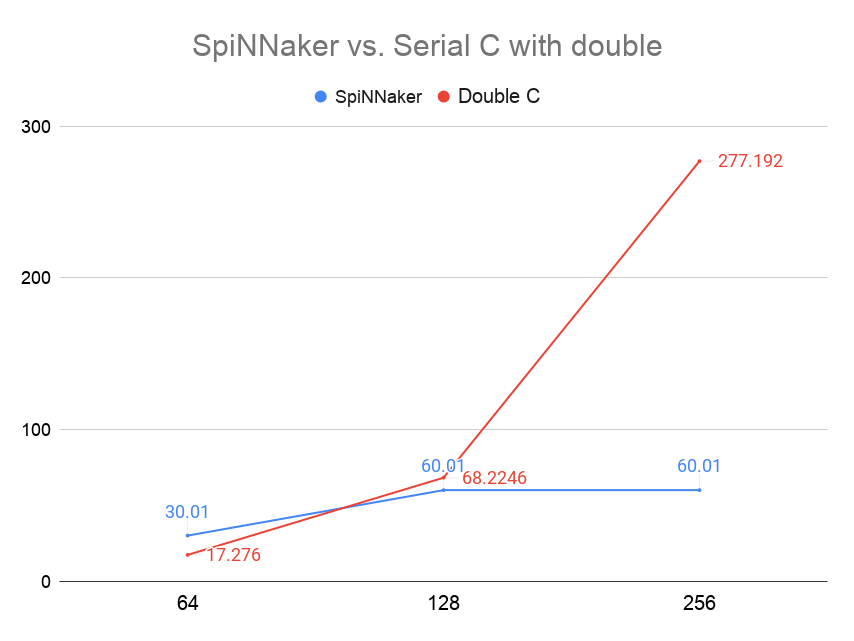
\includegraphics[width=0.8\textwidth]{figures/SpiNNaker vs. Serial C with double.png}
       \caption{Execution time of 12000 time steps in scale of $64\times64$, $128\times128$ and $256\times256$ with SpiNNaker implementation and serial implementation.}
       \label{fig:performance}
\end{figure}

As Fig.~\ref{fig:performance} shows, as the size of the simulation increases, the execution time of the serial program increases rapidly. When the simulation size is small, the serial program executes more efficiently than SpiNNaker; however, as the task size increases, the SpiNNaker naturally implementation utilizes more cores and gets better performance accordingly. For $128\times128$ simulation, the SpiNNaker gain $277.192 / 60.01 = 4.61$ speed-up. With this implementation and hardware, we achieve a relatively good weak-scaling performance.\\

It is noticeable that in SpiNNaker $128\times128$ simulation and $256\times256$ simulation need the same amount of time. This is because: (1) in this project, we only allocate 1 lattice per core. And as the scale of simulation increase, the SpiNNaker implementation will correspondingly increased use of cores; (2) in this project, we have not yet get the optimal performance of SpiNNaker, especially for $128\times128$ simulation. To get a better performance, we are supposed to adjust the SpiNNaker configuration, e.g. timer offset, time scale factor, delay between multicast, really carefully, which need time that beyond the scope of this project.


\subsection{Limitation Analysis} \label{sec:ana}
The first limitation is from the device itself. In the previous performance analysis, we only take the time spend on \textbf{simulation}, which means we do not take the non-simulation time ,e.g. booting the machine, loading data specification to the device, loading data back to host etc., into account. In fact, with the increasing scale of the simulation, the time spend on the non-simulation tasks become larger; see \ref{fig:loading}.

\begin{figure}[tb]
   \centering
       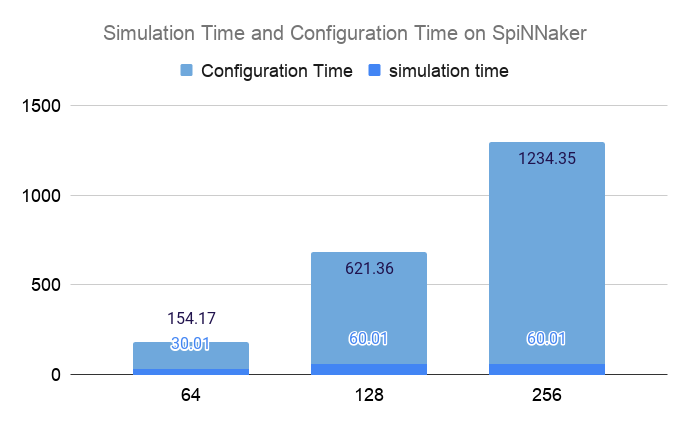
\includegraphics[width=0.8\textwidth]{figures/Simulation Time and Configuration Time on SpiNNaker.png}
       \caption{Simulation time and the configuration time for three different scale simulation. From the chart, it is clear that as the increasing of the simulation scale, there are more time spending on setting up the device and get the simulation result back to host.}
       \label{fig:loading}
\end{figure}

At the moment, it's not possible to solve the problem completely, because as the increasing of simulation scale, there will be more data need to transfer before and after the simulation. However, a group of researchers and engineers are working on tools that enable the SpiNNaker to load data in parallel, which would accelerates data transfer greatly.

Another limitation is that, in this project, we only allocate 1 lattice per SpiNNaker core. Although, we can get parallelism from this configuration, the number of available cores significantly limits the upper limit of simulation scale. In this implementation with available SpiNNaker hardware (about 1,000,000), the maximum scale of simulation is around  $1000 \times 1000$, which is not yet sufficient for real-world engineering problems.